In this chapter we report the results of the training and validation of the neural networks described in the experimental approach. Then, we discuss the results in terms of the research questions defined. Lastly, we assess the limitations of our experimental procedure and results

\section{Experiment Result}
\begin{table}	
	\centering
	\begin{tabular}{ |c|c|c|c|c| } 
		\hline
		& MNIST & Fashion MNIST & CIFAR-10 & SVHN \\ 
		\hline
		LeNet-5	& 0.9834 & 0.8816 & 0.6561 & 0.809\\
		\hline 
		VGG-like & 0.9946 & 0.91 & 0.4075 & 0.067\\ 
		\hline
		Resnet20v1 & 0.9246 & 0.592 & 0.7567 & 0.866\\ 
		\hline
		Resnet20v2 & 0.9222 & 0.8425 & 0.679 & 0.893\\
		\hline
		SqueezeNet & 0.9858 & 0.8813 & 0.555 & 0.775\\
		\hline
	\end{tabular}
	\caption{Accuracy table}
	\label{tab:accuracy}
\end{table}

\begin{table}
	\centering
	\begin{tabular}{ |c|c|c|c|c| } 
		\hline
		& MNIST & Fashion MNIST & CIFAR-10 & SVHN \\ 
		\hline
		LeNet-5	& 220s & 220s & 330s & 220s\\
		\hline 
		VGG-like & 4986s	& 4469s & 6816s & 6526s\\ 
		\hline
		Resnet20v1 & 7970s & 7909s	& 7204s & 9310s\\ 
		\hline
		Resnet20v2 & 13900s & 	13910s & 	12060s & 	15693s\\
		\hline
		SqueezeNet & 13800s & 	13907s & 	13630s & 	17550s\\
		\hline
	\end{tabular}
	%\caption{Execution time for each experiment.}
	\caption{Execution time table}
	\label{tab:times}
\end{table}
Table \ref{tab:accuracy} shows the result of the experiments in terms of accuracy. The execution times and number of parametes for each experiment is shown on Table \ref{tab:times} and Figure \ref{fig:params} respectively. 

\begin{figure}[h]
	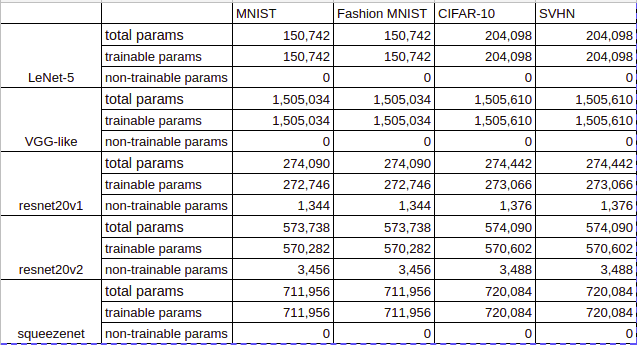
\includegraphics[scale=0.5]{figures/params}
	\centering
	\caption{Number of parameters for each experiment.}
	\label{fig:params}
\end{figure}

\section{Discussion}
In this section, we discuss results of the experiments to answer the following research questions that was previously stated: "How does the performance comparison of deep learning architecture model looks like for a given image classification dataset?"
From the execution time, it is shown that LeNet is the fastest network to train (around 22 seconds/epoch) followed by Simplified VGG-Net, Resnet20V1. ResNet20V2 and SqueezeNet are the most time consuming network to train. LeNet is also the least memory consuming network, followed by ResNet20V1, ResNet20V2, SqueezeNet and Simplified VGG network respectively. In terms of accuracy, there are no single architecture that produces the best result for each datasets. Then, we still need to answer these following additional research questioned that was stated earlier. 

\begin{enumerate}
	\item Which architecture that works bests for a given datasets?
	
	From table \ref{tab:accuracy}, we can see that Simplified VGG architecture performs best on MNIST and Fashion MNIST dataset. ResNet20V1 and ResNet20V2 performs best on CIFAR-10 and SVHN dataset respectively. In terms of memory usage and time consumption, it is shown that LeNet produces the simplest network for all datasets.
	
	\item What kind of datasets characteristics that makes a deep learning architecture works well?
	
	From table \ref{tab:accuracy}, we can see that LeNet generally works well across all dataset except CIFAR-10. With a low amount of training time and low memory consumption, this network can be an initial tester for classifying an image dataset.
	
	Simplified VGGNet performs well on grayscale dataset: MNIST and Fashion-MNIST but gives low accuracy for colored dataset: CIFAR-10 and SVHN dataset. This is an indication that maybe VGG-like architecture performs better on grayscale dataset compared to colored dataset. Also since CIFAR-10 and SVHN image size are bigger than MNIST and Fashion-MNIST, it could be an indication that Simplified VGG-Net works better on smaller image dataset.
	
	ResNet20v1 gives high accuracy in digit recognition dataset: MNIST and SVHN but performs worse on object recognition dataset: Fashion-MNIST and CIFAR-10. It could be that the architecture is suitable for digit recognition dataset compared to object-recognition dataset.
	
	ResNet20v2 which is a refinement from ResNet20v1 does not always increase the performance of ResNet20v1. However, on Fashion MNIST dataset, the improvemance is quite huge, around 25\% accuracy. This architecture gives the most stable performance compared to other architecture, with the lowest accuracy is 67.9\% on CIFAR-10 dataset.
	
	SqueezeNet is the most time consuming network to train, however it does not yields the best solution for any dataset. We need to test it on bigger epoch and see whether it can produces better result or not. If it is indeed yields a better result, then we could say that this architecture has slow improvement rate for every epoch. If is not, then we could say that this architecture is not suitable for these datasets.
	
	\item Is there any architecture that generally works well for image classification?
	
	There are no single architecture that gives best performance across all datasets. However, based on table \ref{tab:accuracy} we can see that in general, ResNet20v2 gives the most stable and good performance on average across all datasets. This does not means that this architecture always gives stable and good performance on most datasets. Further experiment needs to be done to confirm this findings.
	
		
\end{enumerate}

\section{Limitation}
Due to the time and hardware contraint, this studies was conducted only on 4 datasets and 5 architectures. A more powerful machine/hardware is needed to do further benchmarking studies. As an example, applying ResNet20V1 on CIFAR-10 dataset, using current machine took 720 seconds/epoch while applying it on GTX1080Ti took 35 seconds/epoch (according to \href{https://github.com/keras-team/keras/blob/master/examples/cifar10\_resnet.py}{https://github.com/keras-team/keras/blob/master/examples/cifar10\_resnet.py}). Faster experiment means better classification performance and more architecture and dataset that could be implemented. 